\subsection{Método TAMA}

% \begin{frame}
%   \frametitle{Problema del alineamiento de tiempo}

%   \begin{figure}[t]
%     
\includegraphics[scale=0.40]{images/conversation_turns.pdf}
%   \end{figure}
%   Uno de los problemas que tenemos a la hora de construir métricas de mimetización

%   \begin{itemize}
%     \item ¿Cómo comparamos los diferentes turnos de una conversación?
%     \item Comparar uno a uno es un enfoque simplista y no representativo de la realidad
%   \end{itemize}
% \end{frame}



\begin{frame}
  \frametitle{Método TAMA}
  \framesubtitle{Time Aligned Moving Average}
  \begin{itemize}
    \item Introducido en Kousidis et al (2008) \footnote{Spyros Kousidis, David Dorran, Ciaran McDonnell, and Eugene Coyle. Times series analysis of acoustic feature convergence in human dialogues. In
Proceedings of Interspeech, 2008.}
    \item Construímos en primer lugar series de tiempo para cada uno de los hablantes, dada una variable acústico/prosódica.
    \item Mimetización se define como una función de estas dos series.
  \end{itemize}
\end{frame}


\begin{frame}
  \frametitle{Series de Tiempo}
  \framesubtitle{¿Qué es una serie de tiempo?}

  \begin{figure}[t]
    \includegraphics[scale=0.35]{images/oil_price.jpg}
  \end{figure}

  \begin{itemize}
     \item En términos coloquiales, una serie de tiempo es una colección de datos temporales.
     \item El tipo de análisis que vamos a efectuar es propio de Economía y Ciencias de la Atmósfera.
     \item ¡Mucho más manejables que una sucesión de turnos!
   \end{itemize}
\end{frame}



\begin{frame}
  \frametitle{Método TAMA}
  \framesubtitle{Cómo construyo la serie de tiempo (dada una variable a-p)}

  \begin{columns}
    \column{0.50\textwidth}
    \begin{figure}[t]
      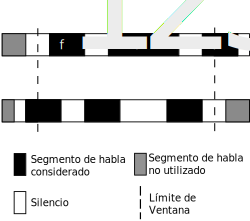
\includegraphics[width=\textwidth]{images/tama_improved.pdf}
    \end{figure}

    \column{0.50\textwidth}
    \begin{enumerate}
      \item Partimos la conversación en ventanas solapadas.
      \item Para cada ventana: calculamos un promedio ponderado del valor de la variable acústico-prosódica en cada segmento de habla
    \end{enumerate}

    \begin{align*}
      \mu = \sum\limits_{i=1}^N f_i \frac{d_i}{D} \text{ con } D = \sum\limits_{i=1}^N d_i
    \end{align*}
  \end{columns}

\end{frame}


\begin{frame}
  \frametitle{Método TAMA}
  \framesubtitle{¿Y la mimetización?}
  \begin{columns}
  \column{0.33\textwidth}

  \begin{figure}[t]
    \includegraphics[scale=0.33]{images/time_plot.png}

    \includegraphics[scale=0.33]{images/cross_correlogram.png}
  \end{figure}

  \column{0.66\textwidth}
  \begin{enumerate}
    \item Ya tenemos la serie de tiempo
    \item ¿Cómo calculamos la mimetización?
    \item Función de correlación cruzada: mide la influencia de una serie sobre otra.
    \item Los valores significativos de esta son los que se consideran los valores de \emph{mimetización} (si es que los hay)
  \end{enumerate}

  \end{columns}
\end{frame}


\subsection{Corpus}
\begin{frame}
  \frametitle{Columbia Games Corpus}
  \framesubtitle{Descripción}
  \begin{columns}
    \column{0.35\textwidth}
      \begin{figure}
        \includegraphics[height=100px,width=\textwidth]{images/columbia_games_color.jpg}
      \end{figure}

    \column{0.65\textwidth}

    \begin{itemize}
      \item Desarrollado por Agustín Gravano para su tesis doctoral.
      \item Corpus de conversaciones diádicas en Inglés Norteamericano
      \item 12 sesiones con 14 tareas/juegos cada una.
      \item En cada sesión, se sentó a dos participantes en una cabina profesional de grabación, y una cortina opaca colgando entre ellos para evitar la comunicación visual.
      \item Los participantes contaron con computadoras a través de las cuales interactuaban mediante juegos.
    \end{itemize}
  \end{columns}
\end{frame}


\begin{frame}
  \frametitle{Columbia Games Corpus}
  \framesubtitle{Anotaciones sociales}

  Cinco anotadores escucharon el audio correspondiente a una tarea del juego y respondieron a varias preguntas sobre los sujetos:


\begin{table}
\adjustbox{max width=0.8\textwidth}{
\begin{tabular}{|l|l|}
  \hline

  \textbf{Nombre} & \textbf{Pregunta} \\
  \hline

  \svcontributes &  ¿el sujeto contribuye para el éxito del equipo?  \\ \hline
  \svengaged &  ¿el sujeto parece comprometido con el juego? \\ \hline
  \svclear &  ¿el sujeto se expresa correctamente? \\ \hline
  \svplanning &  ¿el sujeto piensa lo que va a decir? \\ \hline
  \svencourages &  ¿el sujeto alienta a su compañero? \\ \hline
  \svdifficult &  ¿el sujeto le hace difícil hablar a su compañero? \\ \hline
  \svbored &  ¿el sujeto está aburrido con el juego? \\ \hline
  \svdislikes &  ¿al sujeto no le agrada su compañero? \\ \hline
\end{tabular}
}
\end{table}

De cada una de estas preguntas obtenemos un puntaje de 0 a 5, para cada hablante de cada tarea.
\end{frame}


\begin{frame}
\frametitle{Extracción de features acústico-prosódicas}

Usando el software Praat \footnote{http://www.fon.hum.uva.nl/praat/} se extrajeron las variables acústico-prosódicas para cada segmento de habla

\begin{table}
\adjustbox{max width=0.8\textwidth}{
\centering
\begin{tabular} {|c|c|}
  \hline
  Variable & Descripción \\
  \hline
  \FOMEAN & Valor medio de la frecuencia fundamental \\\hline
  \FOMAX  & Valor máximo de la frecuencia fundamental \\\hline
  \ENGMEAN & Valor medio de la intensidad \\\hline
  \ENGMAX & Valor máximo de la intensidad \\\hline
  \NOISETOHARMONICS & Noise-to-harmonics ratio \\\hline
  \LOCALSHIMMER & Shimmer medido \\\hline
  \LOCALJITTER  & Jitter medido \\\hline
  \SYLAVG & Cantidad de sílabas por segundo \\\hline
  \PHONAVG & Cantidad de fonemas por segundo \\\hline
\end{tabular}
}
\end{table}
\end{frame}



\subsection{Modificaciones a TAMA}


\begin{frame}
\frametitle{TAMA}
\framesubtitle{Nuestra medida de mimetización}

  \begin{columns}
    \column{0.33\textwidth}
    \begin{figure}[t]
      \includegraphics[scale=0.33]{images/time_plot.png}

      \includegraphics[scale=0.33]{images/cross_correlogram_2.png}
    \end{figure}

    \column{0.66\textwidth}

    Definimos dos medidas de mimetización

    \begin{align*}
      \fwentrainment{AB}^{(1)} &= \argmax_{\{r_k, k \leq 0\}} |r_k|  \\
      \fwentrainment{BA}^{(1)} &= \argmax_{\{r_k, k \geq 0\}} |r_k|  \\
      \fwentrainment{XY}^{(2)} &= |\fwentrainment{XY}^{(1)}|
    \end{align*}

    \begin{itemize}
      \item  Segunda métrica motivada por estudios sobre la antimimetización. Healey et al (2014) sugiere que puede ser una conducta de adaptación cooperativa.
      \item  Levitan et al (2015) da más indicios en esa dirección.
    \end{itemize}

  \end{columns}
\end{frame}

\begin{frame}
  \frametitle{Mimetización y relación con variables   sociales}

  \begin{itemize}
    \item Llegado a este punto, ya tenemos medidas de mimetización por cada tarea.
    \item Tambien tenemos las anotaciones sociales
    \item ¿Cómo analizamos su relación?
  \end{itemize}

\end{frame}
\subsection{Análisis de la relación con variables sociales}

\begin{frame}
\frametitle{Mimetización y relación con variables sociales}
  \framesubtitle{Análisis de Regresión}

  Para analizar la relación entre las variables sociales ($V$) y nuestras medidas de \emph{mimetización} ($\mathcal{E}$), planteamos un modelo de regresión lineal.

    \begin{equation}
      V_i \sim \beta_1 + \beta_2 \mathcal{E}_i
    \end{equation}

  Nuestra hipótesis es

  \begin{enumerate}
    \item Si $V$ es una variable de carácter positivo, entonces $\beta_2 > 0$
    \item Si $V$ es una variable de carácter negativo, entonces $\beta_2 < 0$
  \end{enumerate}
\end{frame}
